
\begin{figure}[H]
\centering
\begin{subfigure}[b]{0.45\textwidth}
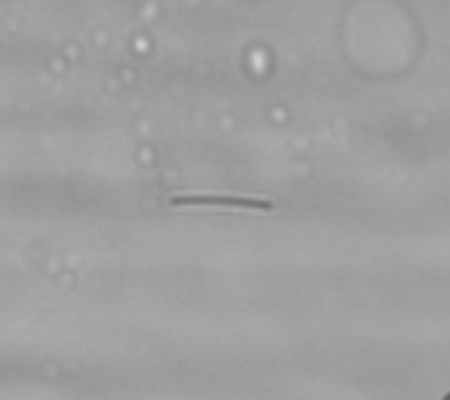
\includegraphics[width=0.9\textwidth]{figures/improvements/oldparticle2.png}
\caption{Particle 13 from July 2012}
\end{subfigure}
\begin{subfigure}[b]{0.45\textwidth}
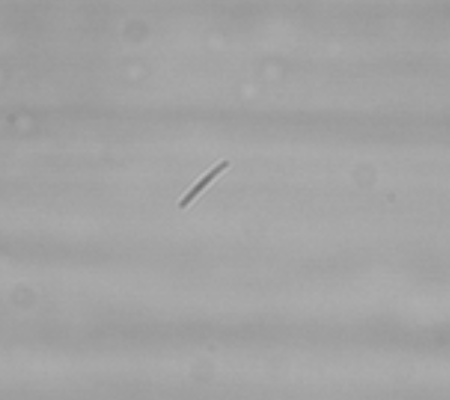
\includegraphics[width=0.9\textwidth]{figures/improvements/oldparticle3.png}
\caption{Particle 22 from July 2012}
\end{subfigure}
\caption{Two fairly typical particles from the previous setup. Note that these are still selected from the total pool of particles for being relatively symmetric and yet are noticeably bent.}
\label{fig:oldparticles}
\end{figure}



To solve the problems with the particles we replaced them with glass particles from Nippon Glass, Japan \cite{Particles}. The particles are made from LCD spacing rods that are , which means they are essentially broken cylinders with very consistend width but quite varying length. Two different batches of particles have been used, one with $3\mu m$ diameter and one batch with $5 \mu m$ diameter. All the particles presented in the results section are from the $3 \mu m$ batch. To verify that the particle were indeed as symmetric and with as even width as we suspected images were taken with an ESEM (Environmental Scanning Electron Microscope) and can be seen in figure \ref{fig:particlepictures}. We see that the particles are uniformly smooth along the edges but have varyingly jagged edges causing different degrees of asymmetry. 

In particular figure \ref{fig:roundparticle} shows a top down view of a particle clearly showing a very circular shape with no discernible asymmetry.

\begin{figure}[H]
\centering
\begin{subfigure}[3a]{0.40\textwidth}
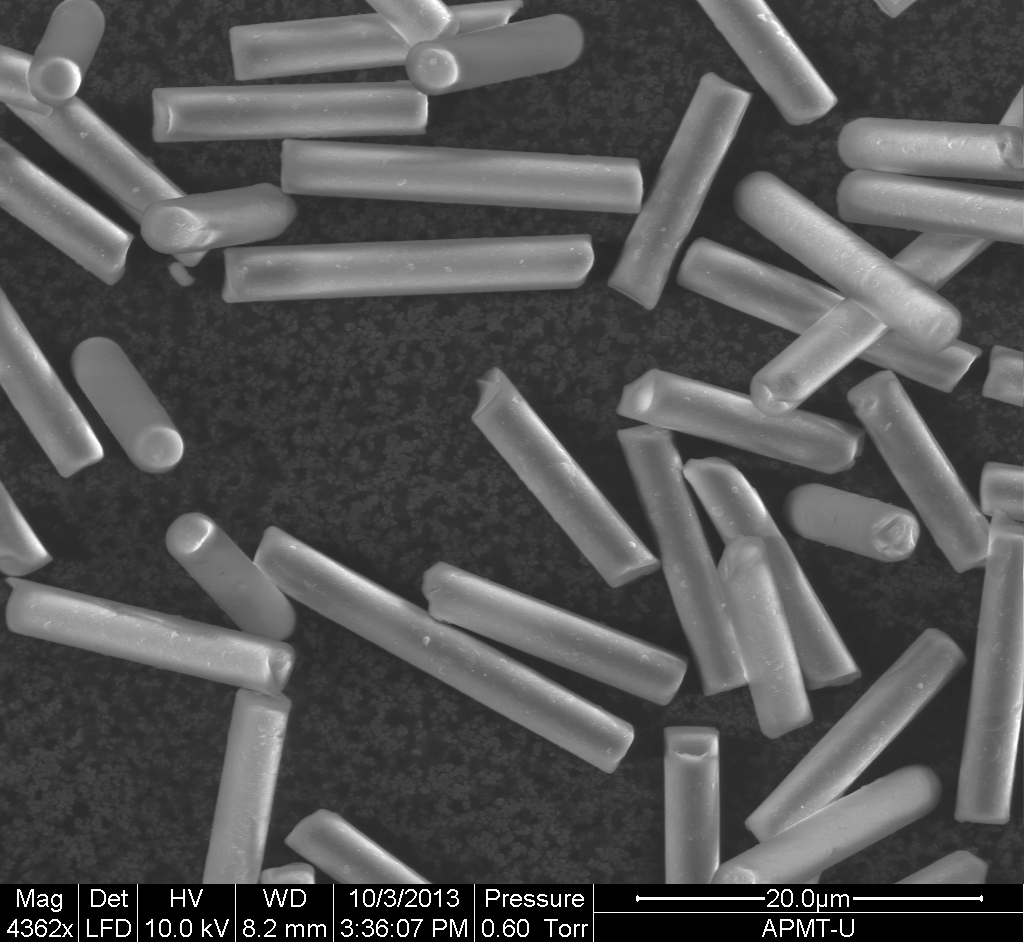
\includegraphics[width=\textwidth]{figures/method/semizoomed.png}
\caption{Shows a detailed view \\ of a number of particles.}
\end{subfigure}\hspace{1em}%
\begin{subfigure}[3b]{0.40\textwidth}
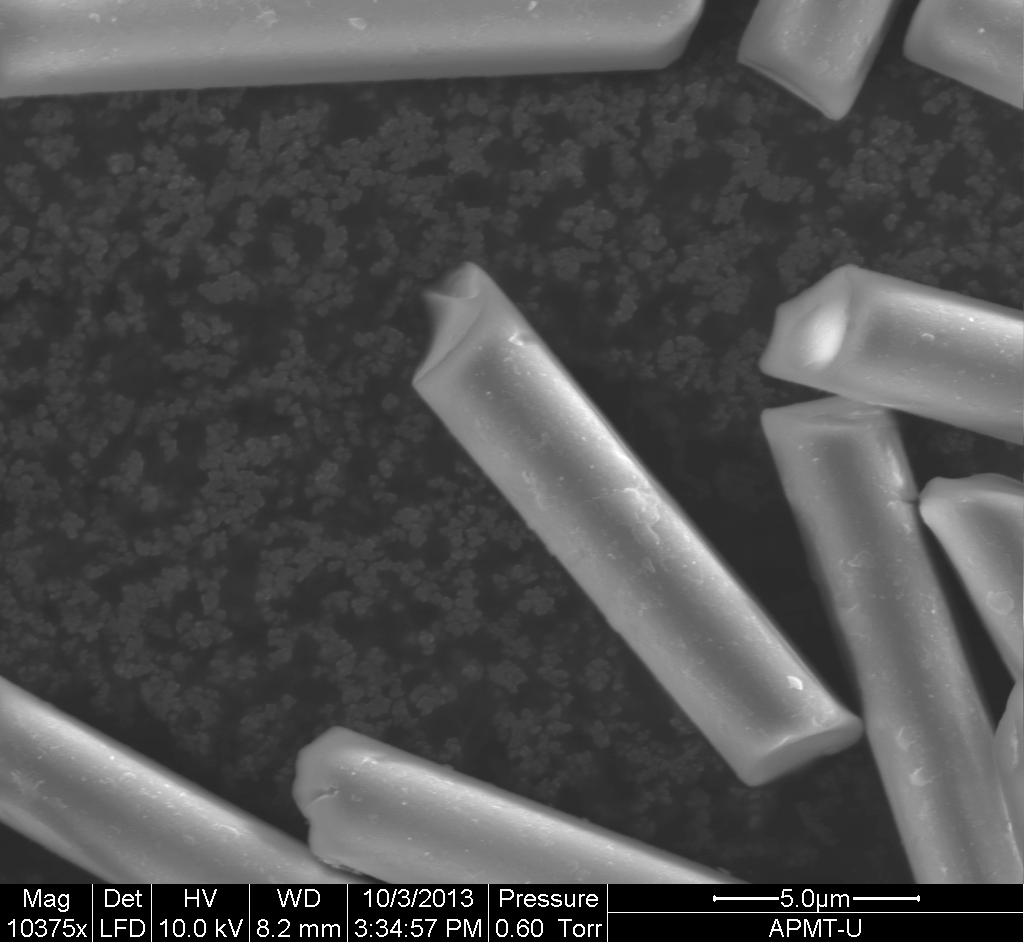
\includegraphics[width=\textwidth]{figures/method/zoomedbroken.png}
\caption{Shows in detail the jagged edge \\ of a particle.}
\end{subfigure}
\caption{Pictures of the glass particles that particles}
\label{fig:particlepictures}
\end{figure}
 
\begin{figure}[H]
\centering
\begin{subfigure}[3a]{0.40\textwidth}
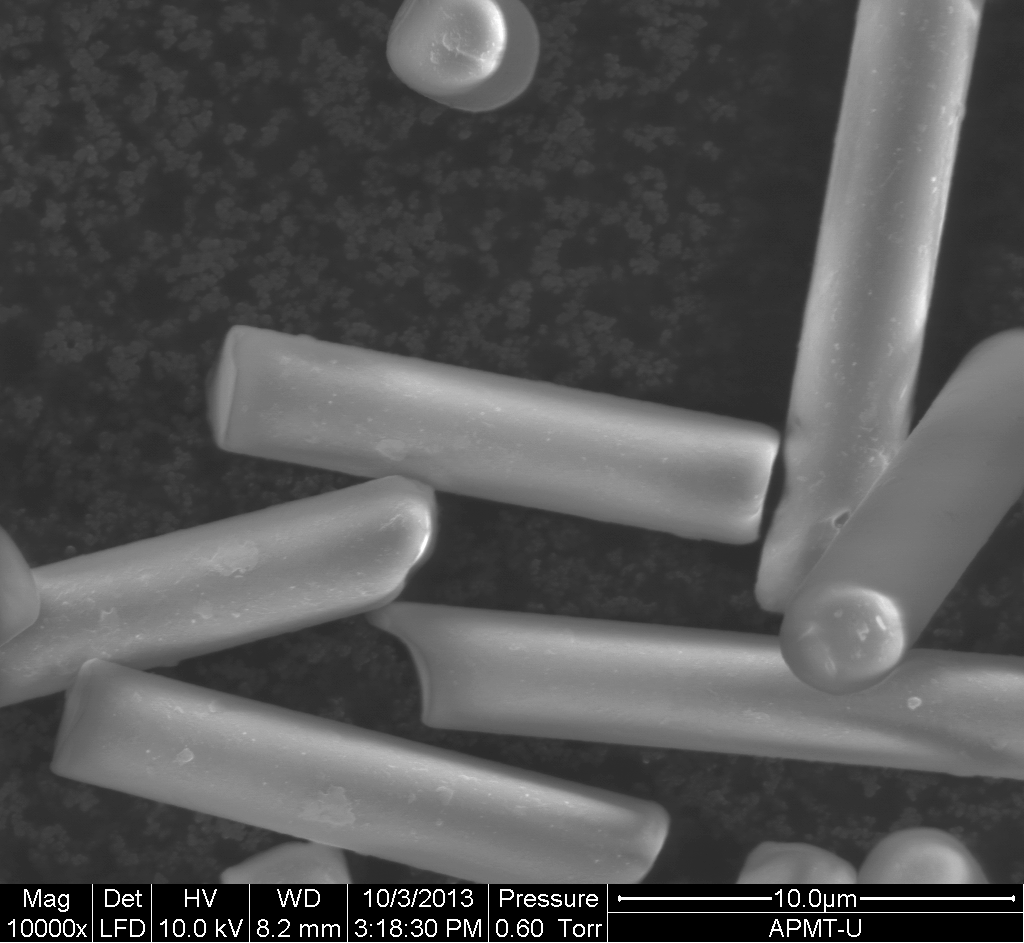
\includegraphics[width=\textwidth]{figures/method/symmetric.png}
\caption{What appears to be a highly \\ symmetric particle.}\label{fig:symmetricparticle}
\end{subfigure}\hspace{1em}%
\begin{subfigure}[3b]{0.40\textwidth}
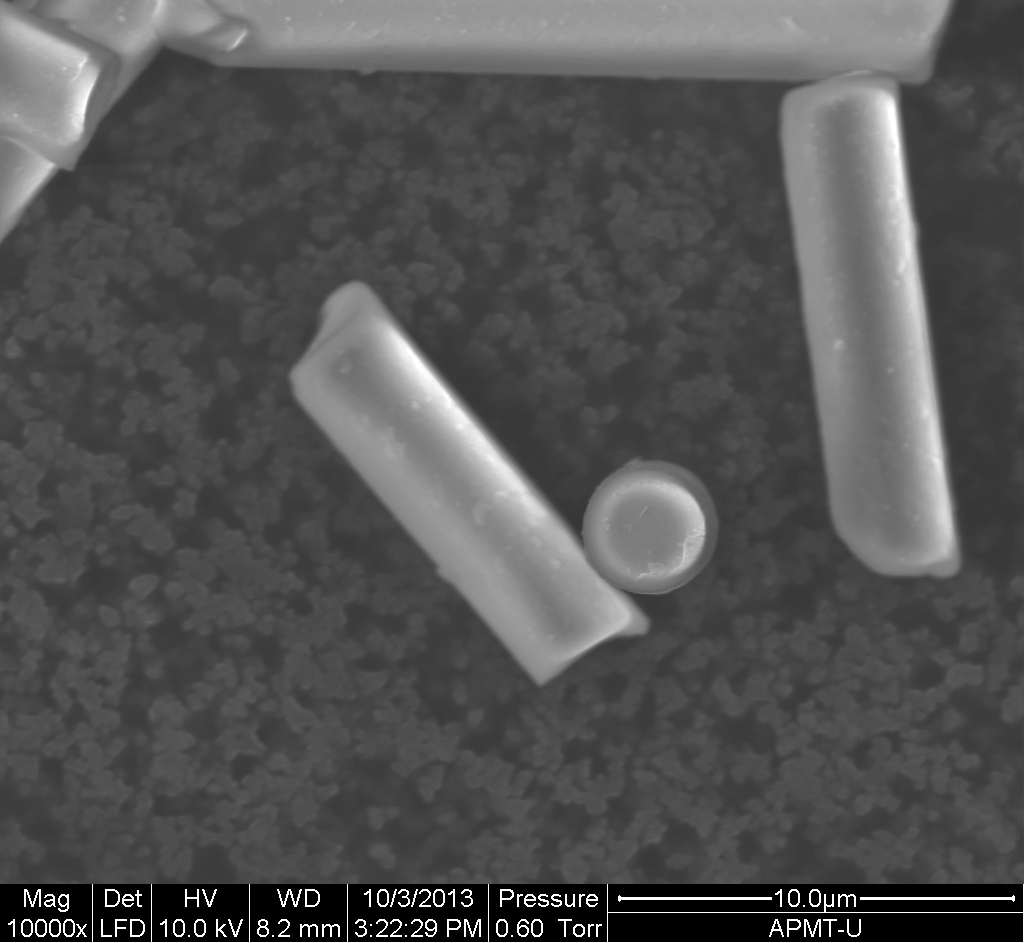
\includegraphics[width=\textwidth]{figures/method/round.png}
\caption{A top down view of a particle.}\label{fig:roundparticle}
\end{subfigure}
\caption{Pictures highlighting the roundness of the particles as well as the apparent symmetry of some particles. It should be noted that altough there are no apparent rough edges there was no way to rotate a sample so there might very well be asymmetries on the side of the particle that we cannot see.}
\label{fig:particlepictures2}
\end{figure}

While these particles seemingly satisfy the symmetry conditions they are made glass with a density of approximately \unit[2.57]{g/cm$^3$} at \unit[20]{C$^\circ$} which is significantly higher than that of water with a density of \unit[1]{g/cm$^3$} at \unit[20]{C$^\circ$} and glycerol with a density of \unit[1.5]{g/cm$^3$}. Thus to correct for the density and limit sinking or floating the water soluble Sodium metatungstate which at \unit[20]{C$^\circ$} has maximum density of \unit[2.94]{g/cm$^3$}. To increase the viscosity of the liquid around 8\% glycerol is added, resulting in a measured dynamic viscosity of \unit[$24\cdot 10^{-3}$]{Pa s}
